\subsection{Other backgrounds from particle misidentification}
\label{sec:db:backgrounds:misid}

Beyond backgrounds from onia states and the \KS decay there are many mesons that decay into a
two-body final state, which could mimic the signal decay given some particle misidentification.
A meson that decays via $\decay{X}{hh^\prime}$ which is then reconstructed
under the incorrect mass hypothesis could pass the selection criteria as either the \db or \Kstarz
candidate.
This type of contamination is studied by assigning different mass hypotheses to each final state
particle and calculating the invariant mass of the \mumu and \kpi candidates.
If the mass of one of these objects, after mass reassignment, is seen to peak at the mass of a
known particle, then the contamination is removed by applying \pid criteria.

Since a selection has been made on the \decay{\Kstarz}{\kpi} candidate using both \pid criteria and
constraints on the \kpi invariant mass it is expected that there will be little contamination
from background sources.
To test this, candidate \Kstarz mesons coming from a \Bd candidate which has an invariant mass
within $80\mev$ of the known \Bd mass are assigned different mass hypotheses to check for peaking
components in the new $\mass{K_{h}^+\pi_{h^\prime}^-}$ mass spectrum.
%\footnote{
  %Where, as defined previously, the notation $h_i$ is a particle under the mass hypothesis of $h$
  %which was reconstructed as an $i$.
%}
The only background that must be removed from this category is from a real \decay{\phi}{\kk}
where a kaon in the final state is misidentified as being a pion.
If the mass of the $\Kp K^-_\pi$ candidate lies within $10\mev$ of the known \phii mass, the
ambiguous pion is subject to the requirements that
$\ProbNN{\pi}<0.3$ and $\ProbNN{K}>0.3$.

Backgrounds from resonances decaying into a pair of hadrons which are then mistaken as a pair of
muons are more problematic.
Misidentification of the decay \decay{\KS}{\pipi} is already dealt with in the preselection, but
there is also contamination from other long-lived hadronic states, namely the \Dz and \Lz.
The decays \decay{\Dz}{\kpi} and \decay{\Lz}{p\pim} are dealt with in a similar way to the vetoes
described in \Sec{sec:dsphi:sel:veto}.
If the invariant mass of the $K^+_\mu\pi^-_\mu(p_\mu\pi^-_\mu)$ candidate falls within $25(10)\mev$
of the nominal $\Dz(\Lz)$ mass, then the muons is subject to the requirement that
$\ProbNN{\mu}(\Kp_\mu,\pip_\mu)>0.3(\ProbNN{p}(p_\mu)<0.3)$.


\begin{table}
  \caption[Misidentification vetoes]
  {
   Vetoes to suppress double and single misidentification of particles.
   If, under the alternate hypothesis, the \db or \Kstarz candidate mass falls within the range
   indicated, the candidates are subject to the given \pid requirements.
  }
  \label{tab:bkg:vetoes}
  \begin{center}
    \begin{tabular}{lcc}\toprule
      \multicolumn{2}{c}{Mass criteria (MeV)} & PID requirement \\\midrule
      $\left|m(\Kp K^-_\pi) - m^\mathrm{PDG}_\phi\right|$ & $<10$
      & $\ProbNN{\pi}(\pi)>0.3$ and \ProbNN{K}$(\pi)<0.3$
      \\\rule{0pt}{3ex}$\left|m(K^+_\mu\pi^-_\mu) - m^\mathrm{PDG}_{\Dz}\right|$& $<25$
      & $\ProbNN{\mu}(\mu)>0.3$
      \\\rule{0pt}{3ex}$\left|m(p_\mu\pi^-_\mu) - m^\mathrm{PDG}_{\Lz}\right|$ & $<10$
      & $\ProbNN{p}(\mu)<0.3$
      \\\rule{0pt}{3ex}$\left|m(p_\pi K^-\mumu) - m^\mathrm{PDG}_{\Lb}\right|$ & $<50$
      & $\ProbNN{p}(\pi)<0.2$  \\
      \bottomrule
    \end{tabular}
  \end{center}
\end{table}

Misidentifying the proton as a pion in the decay \decay{\Lb}{p\Km\mumu} can contaminate the
selected \btokstrdb candidates.
Figure~\ref{fig:db:lb} shows the invariant mass distribution of the $p_\pi\Km\mumu$ system for
candidates where $\ProbNN{p}(p_\pi)>0.2$, a clear peak is observed at the known mass of the \Lb.
To remove this contamination, if the invariant mass of the \Lb candidate falls with $50\mev$ of the
nominal \Lb mass, the candidate is vetoed.


\begin{figure}
  \begin{center}
    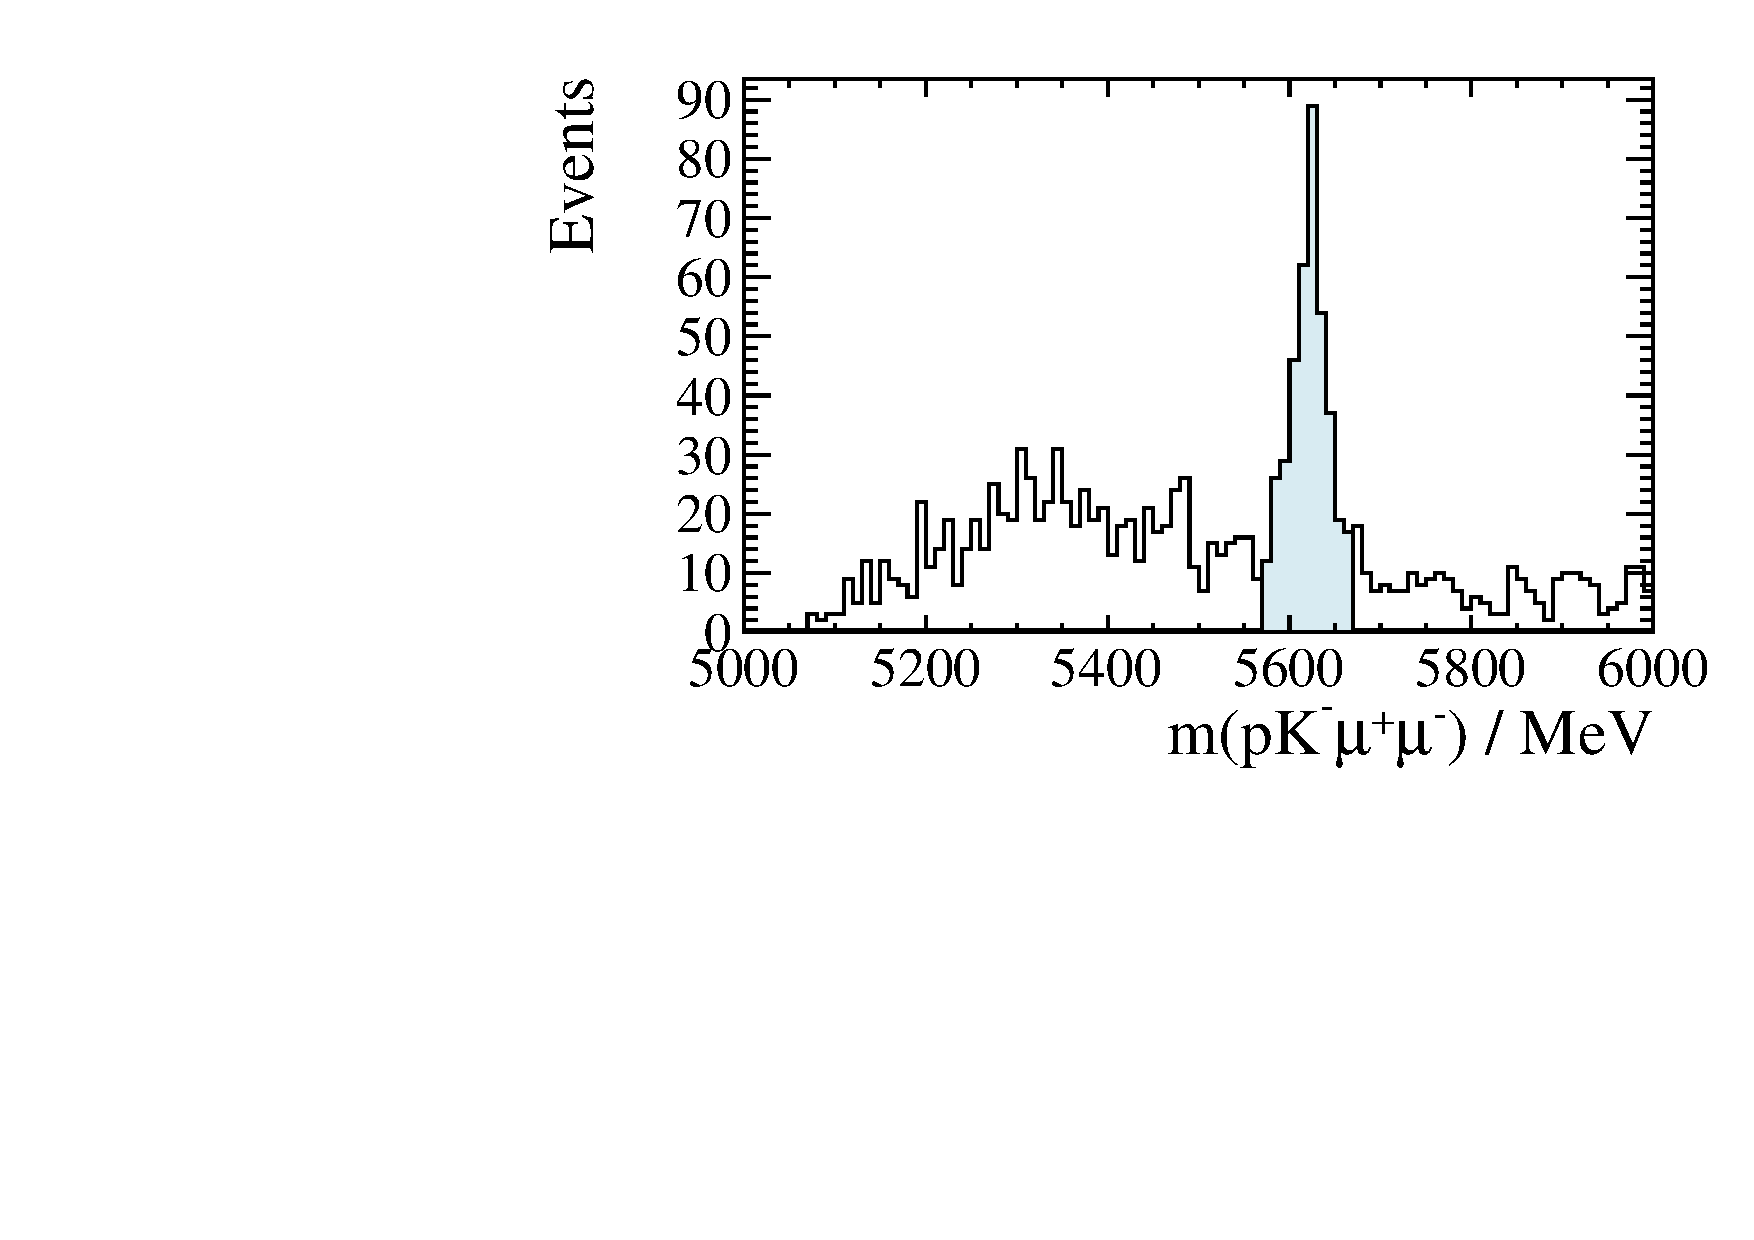
\includegraphics[width=0.48\textwidth]{lb2pkmumu}
    \caption[Contamination from the decay \decay{\Lb}{p\Km\mumu}]
    {
      Contamination from the decay \decay{\Lb}{p\Km\mumu}, where the proton is misidentified as a
      pion, here a cut of $\ProbNN{p}(p_\pi)$ has been applied and a clear peak at the known \Lb
      mass, $5219.4\mev$, is observed.
      Candidates are vetoed if they lie within $50\mev$ of the \Lb mass, which is shown as the
      shaded region.
    }
    \label{fig:db:lb}
  \end{center}
\end{figure}

%There are also contributions from the decay \decay{\Bd}{\jpsi\Kstarz} and \decay{\jpsi}{\mumu},
%where one of the hadron is misidentified as a muon, and vice versa.
%This can be trivially removed by requiring that the hadrons do not satisfy {\tt isMuon}, as shown
%in \Fig{fig:bkg:doublemisid}.

%\begin{figure}
  %\begin{center}
    %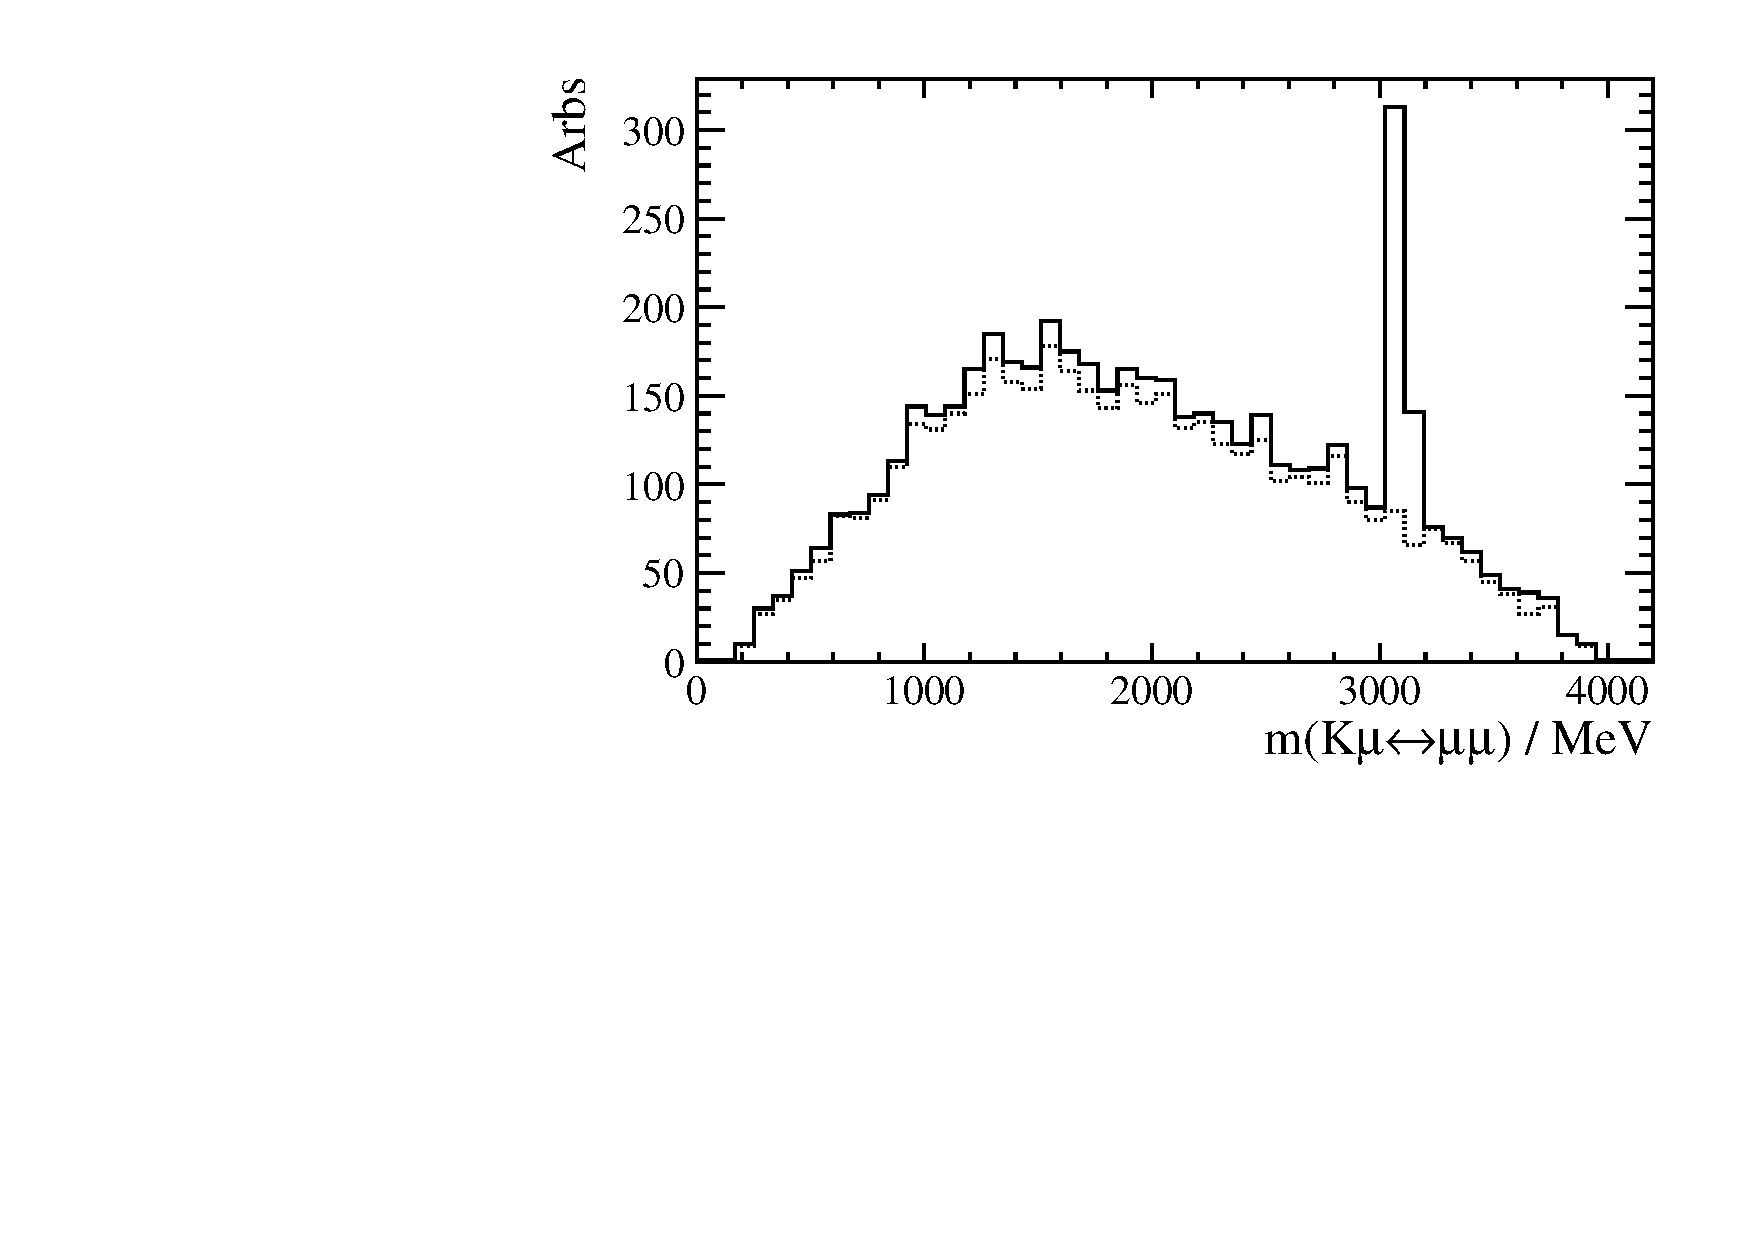
\includegraphics[width=0.48\textwidth]{double_misid_pi}
    %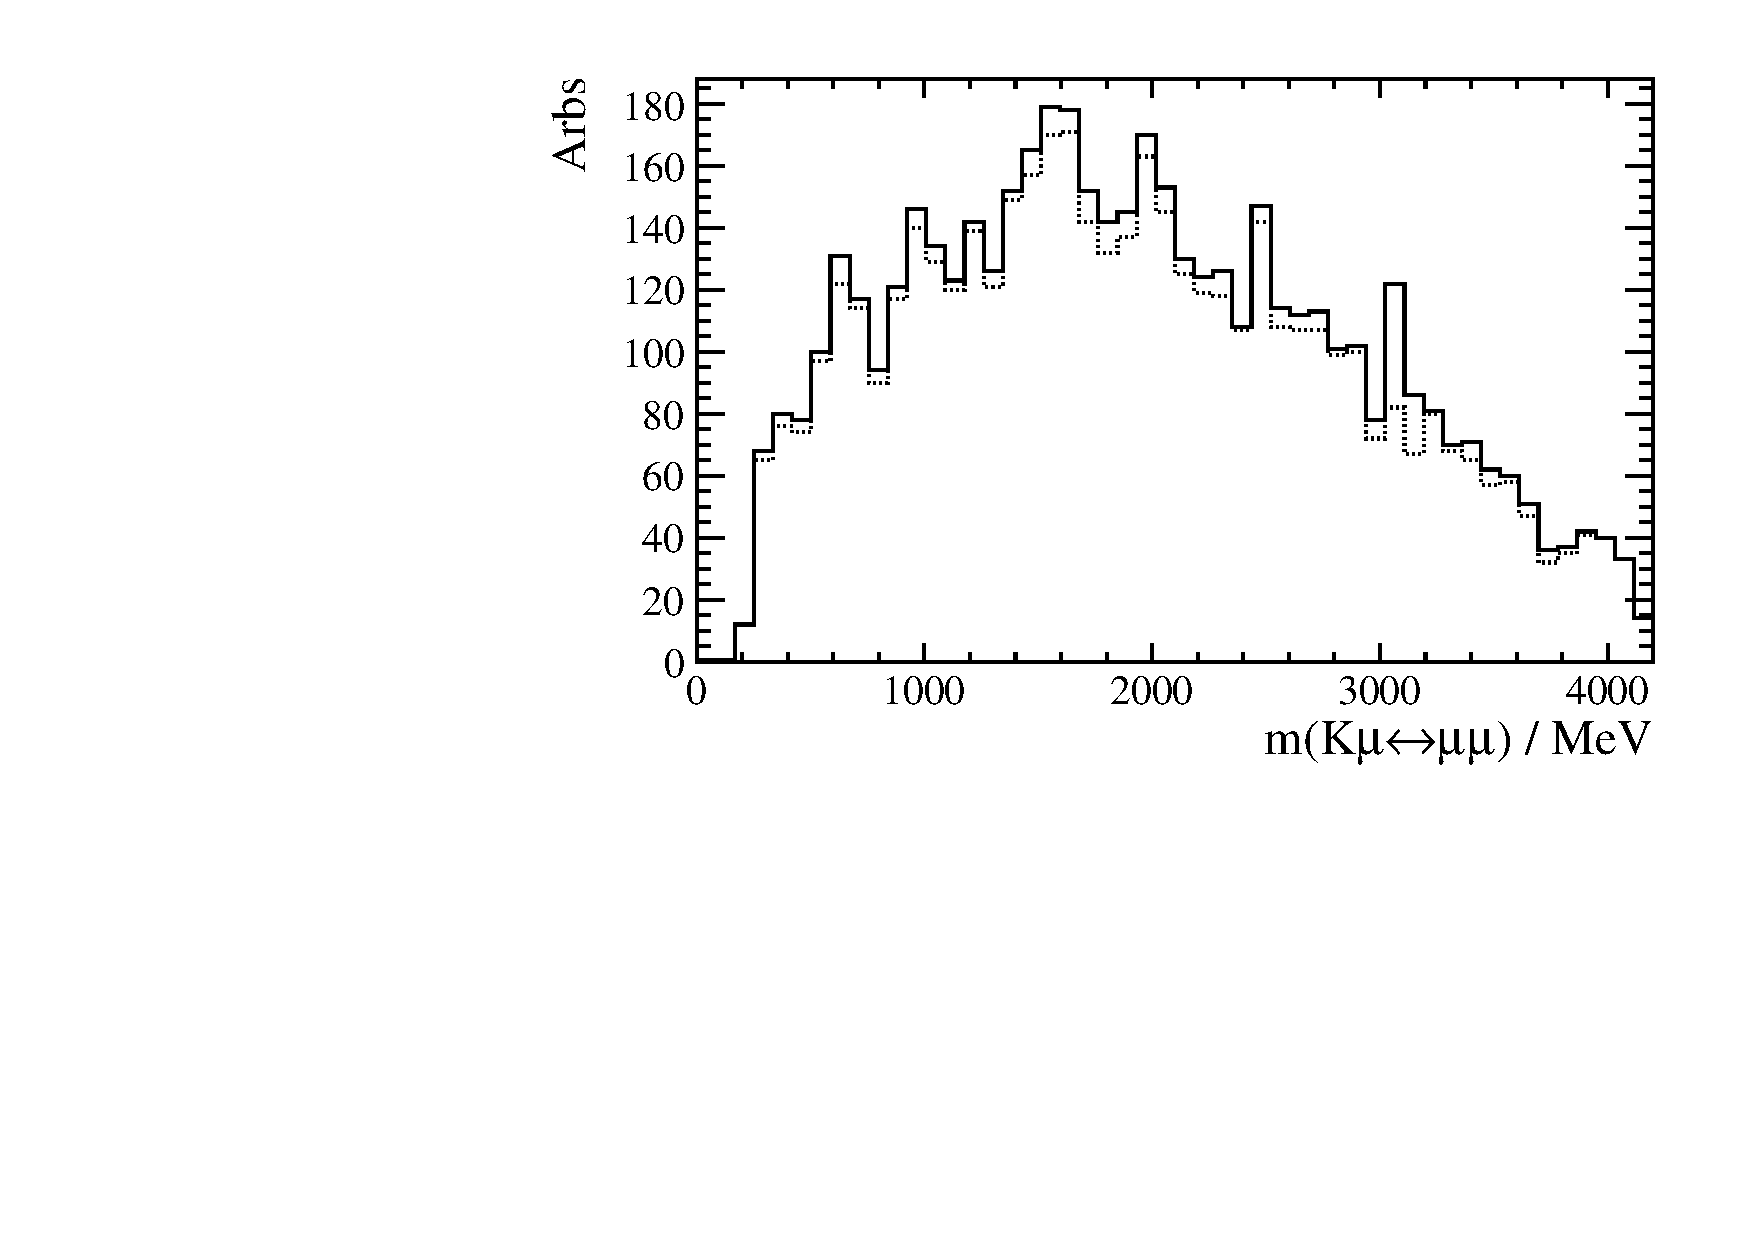
\includegraphics[width=0.48\textwidth]{double_misid_k}
    %\caption{\small
      %Background contributions from \decay{\Bd}{\jpsi\Kstarz}, where both a muon and (left) pion
      %and (right) kaon are misidentified as one another.
      %This background is very effectively removed by requiring that the hadron does not satisfy the
      %{\tt isMuon} criteria; the effect of this veto is shown with a dotted line.
    %}
    %\label{fig:bkg:doublemisid}
  %\end{center}
%\end{figure}

The sidebands are used to estimate the level of background in the signal region.
Therefore, background
contributions are only problematic if they produce a narrow peaking structure in the dimuon mass,
because misidentification causes the $m_{\mumu}$ distribution to be smeared.
In general misidentification is only problematic if the decaying particle has a very narrow natural
width.
Therefore, any remaining misidentification-type backgrounds have negligible effect in the analysis.


%%%%%%%%%%%%%%%%%%%%%%%%%%%%%%%%%%%%%%%%%%%%%%%%%%%%%%%%%%%%%%%%%%%%%%%%%%%%%%%%%%%%%%%%%%%%%%%%%%
\subsection[Possible contamination from the \xtsvty]
{Possible contamination from the $\boldsymbol{\xtsvty}$}
\label{sec:x1070}
%%%%%%%%%%%%%%%%%%%%%%%%%%%%%%%%%%%%%%%%%%%%%%%%%%%%%%%%%%%%%%%%%%%%%%%%%%%%%%%%%%%%%%%%%%%%%%%%%%
While searching for potential backgrounds resulting from misidentifying two hadrons as muons, a
peak was found in the invariant mass spectrum of the $K_\mu^+K_\mu^-$ candidates.
This peak was consistent with the \xtsvty listed in \Ref{PDG2014}, which has a mass of
$(1072\pm1)\mev$ with a width of $(3.5\pm0.5)\mev$ and was observed in the $\KS\KS$ distribution
from a pion beam interacting with a liquid hydrogen target~\cite{x1070vlad}.
%from $\pim p \to \KS \KS n m\piz$ collisions~\cite{x1070vlad}, where $m\in\mathbb{Z}$.
Figure~\ref{fig:x1070} shows the observation of this resonance from \Ref{x1070vlad} alongside
the data from this analysis.

\begin{figure}
  \begin{center}
    %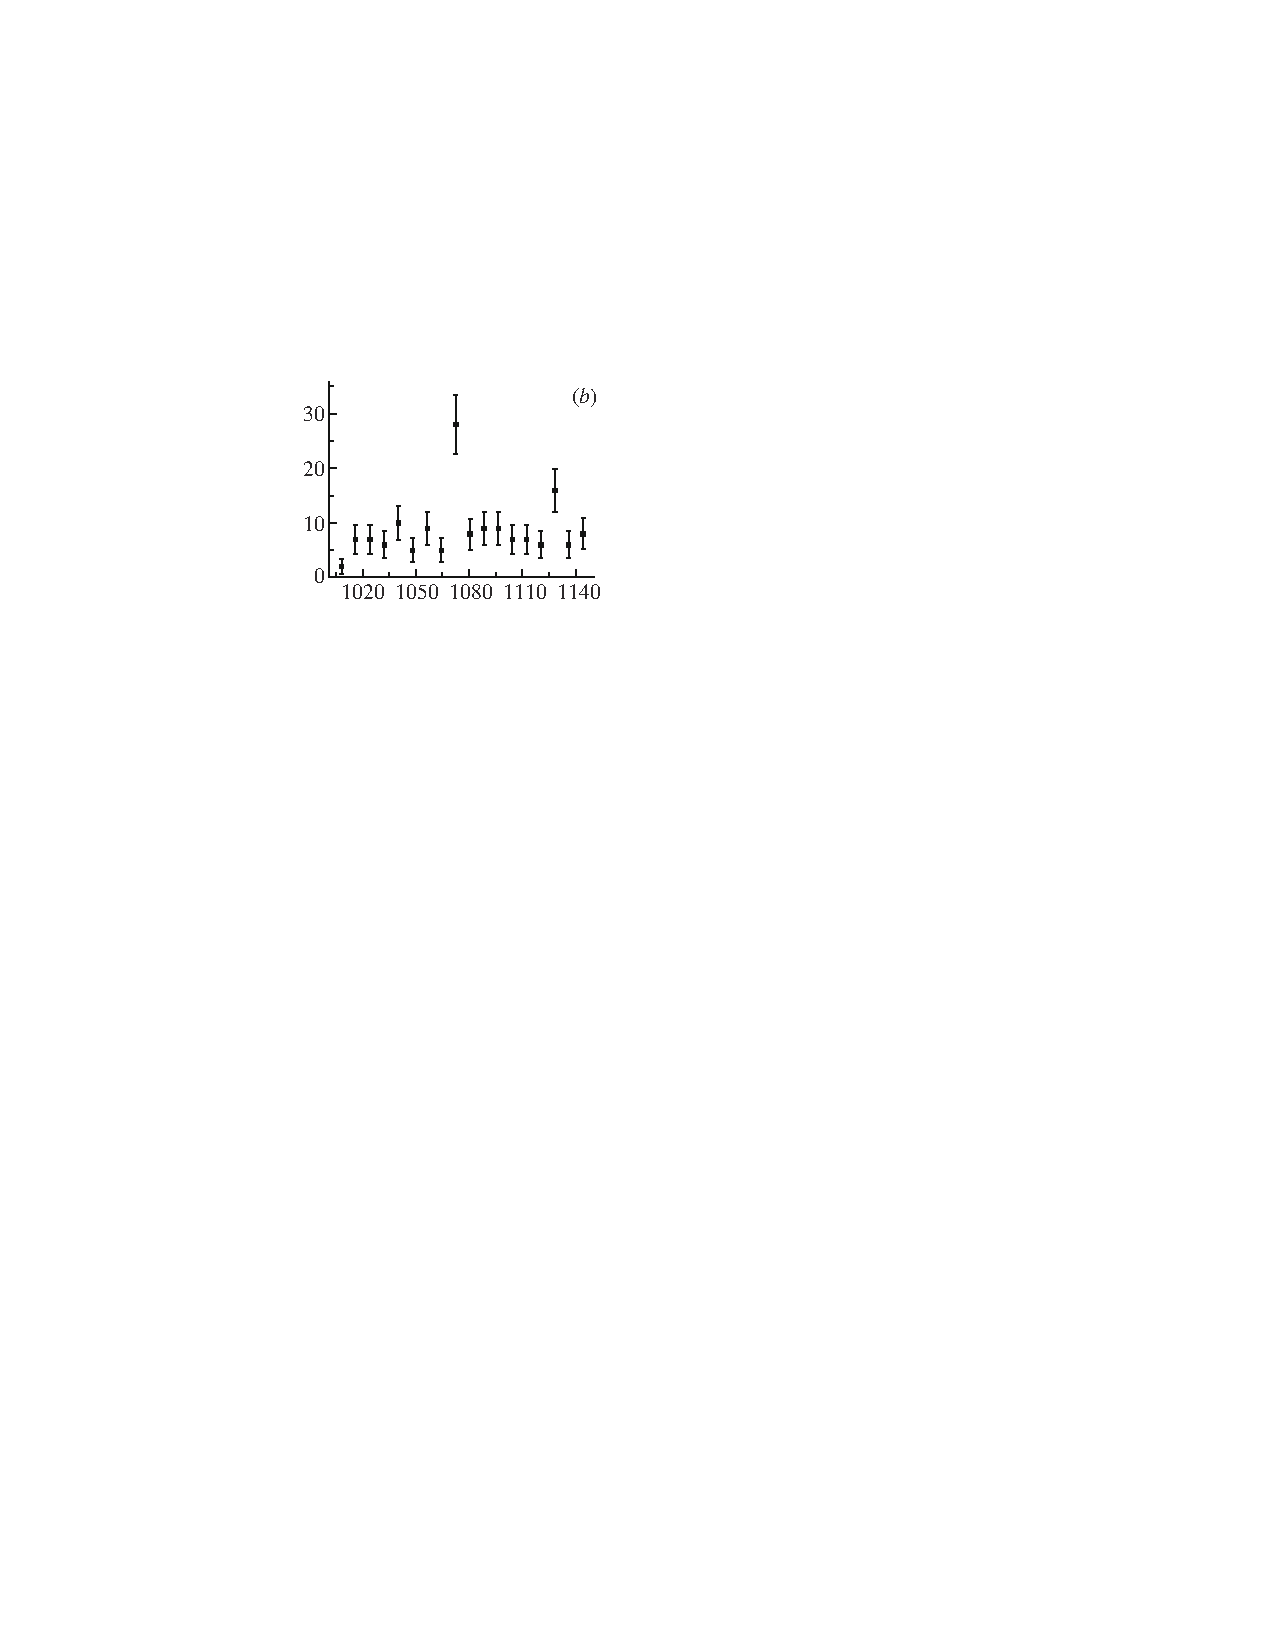
\includegraphics[height=0.2\textheight]{x1070vlad}
    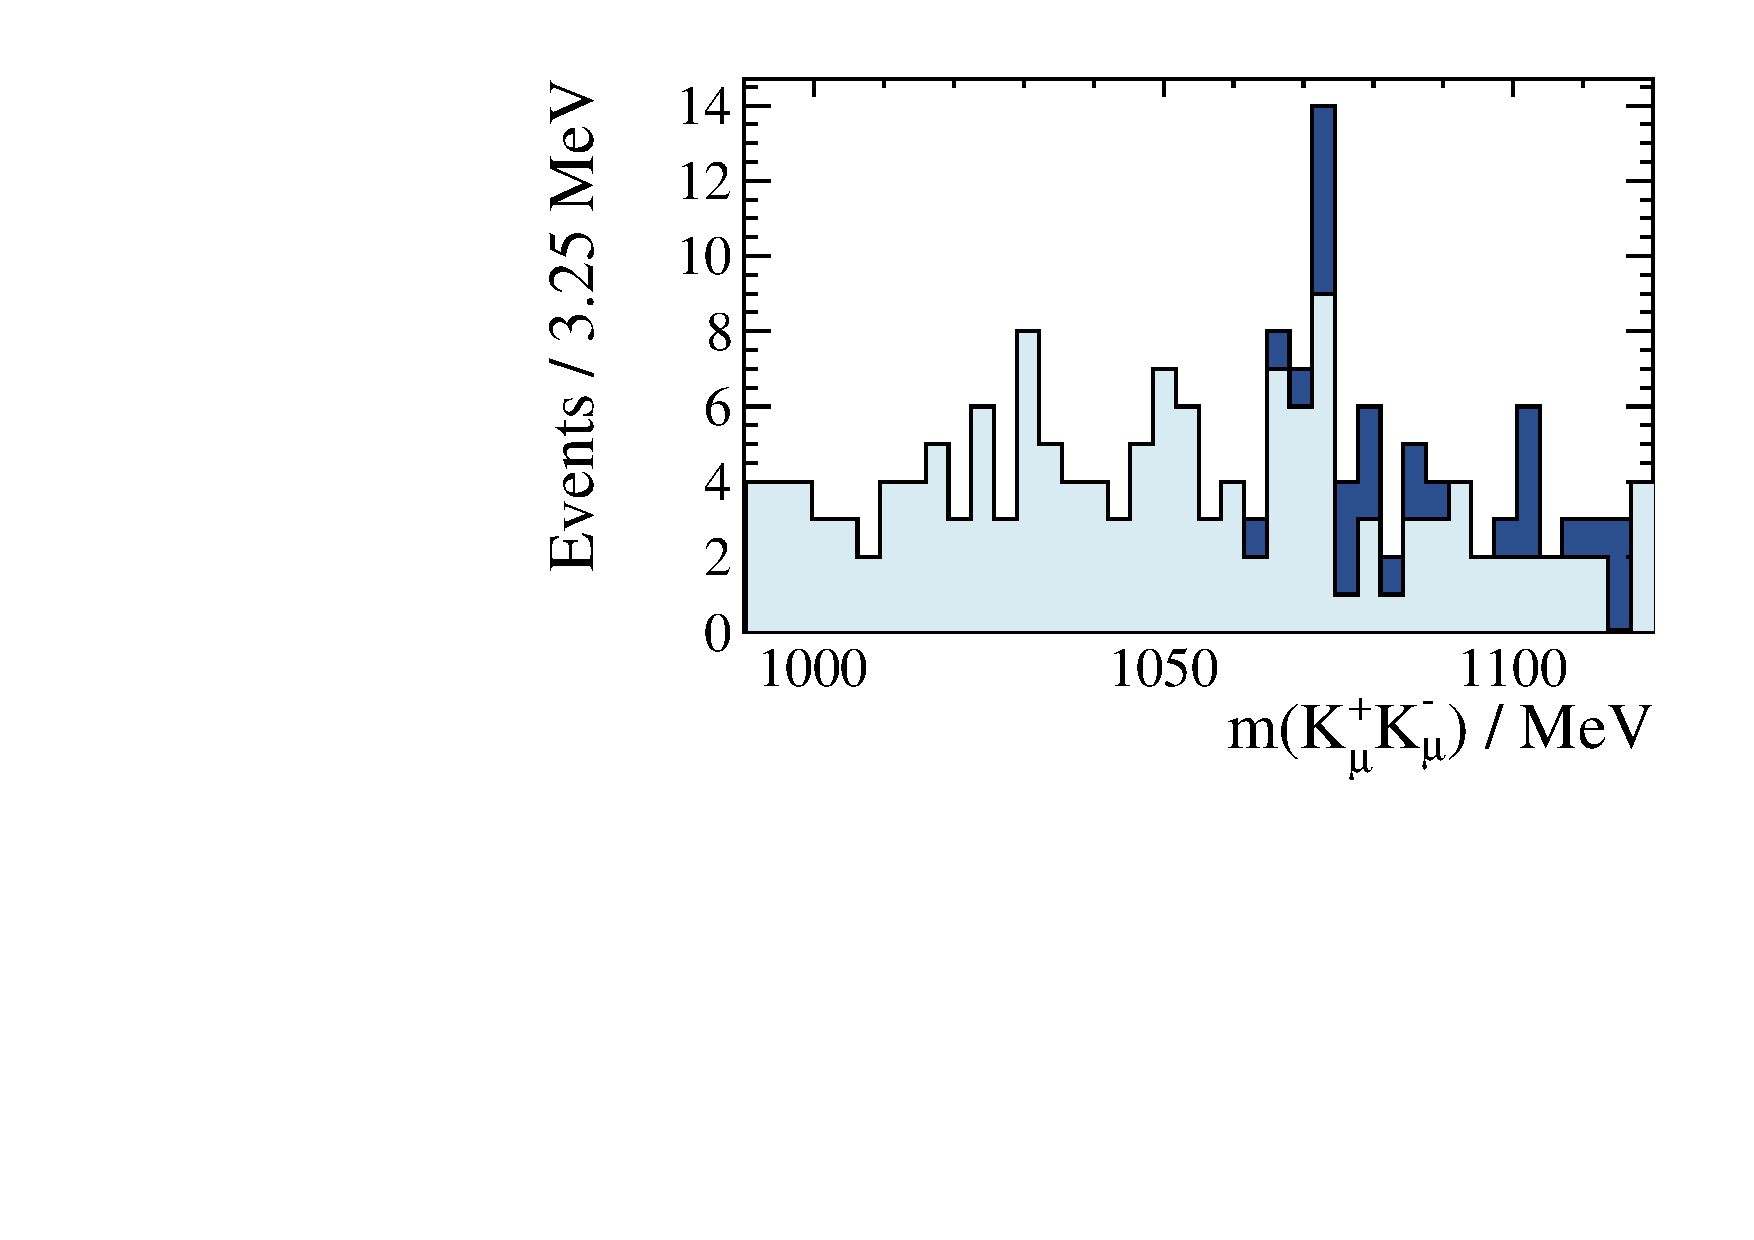
\includegraphics[height=0.2\textheight]{mumu_kk}
    \caption[Invariant mass of the \mumu distribution under the \kk mass hypotheses]
    {
      %A comparison of
      %(left) the data which observes the \xtsvty~\protect\cite{x1070vlad}, and
      Invariant mass distribution of the $K_\mu^+K_\mu^-$ candidates in data, showing a peak at
      \approx$1072\mev$ in data.
      The dashed line indicates the effect of vetoing the decay
      \decay{\KS}{\pip\pim} in the preseletcion.
    }
    \label{fig:x1070}
  \end{center}
\end{figure}

Figure~\ref{fig:db:x1070:2d} shows a comparison of simulated \decay{\KS}{\pipi} decays with the
observed data near this excess.
It is clear that \decay{\KS}{\pipi} decays produce a peak around $1072\mev$ under the \kk
hypothesis.
There is also a long tail but with low statistics and with a roughly uniform
background this tail would not be expected to be visible in the data after the \KS veto in the
preselection.

Initially the \mumu pair under the \kk mass hypothesis appeared to have a contribution from a
decaying \xtsvty.
However, this is not the case, and the peak at $m_{K^+_\mu K^-_\mu}=1072\mev$ is due to the decay
\decay{\KS}{\pipi}.
Removing events satisfying $|\mass{\pi_\mu^+\pi_\mu^-}-m_{\KS}^\mathrm{PDG}|<25\mev$ removes much
of the peak at $1072\mev$, bringing it in line with the background.
Also, the fact that no \decay{\phi}{\kk} is observed in the $m_{K^+_\mu K^-_\mu}$ spectrum
indicates that there this is a false peak and need not be accounted for further.


\begin{figure}
  \begin{center}
    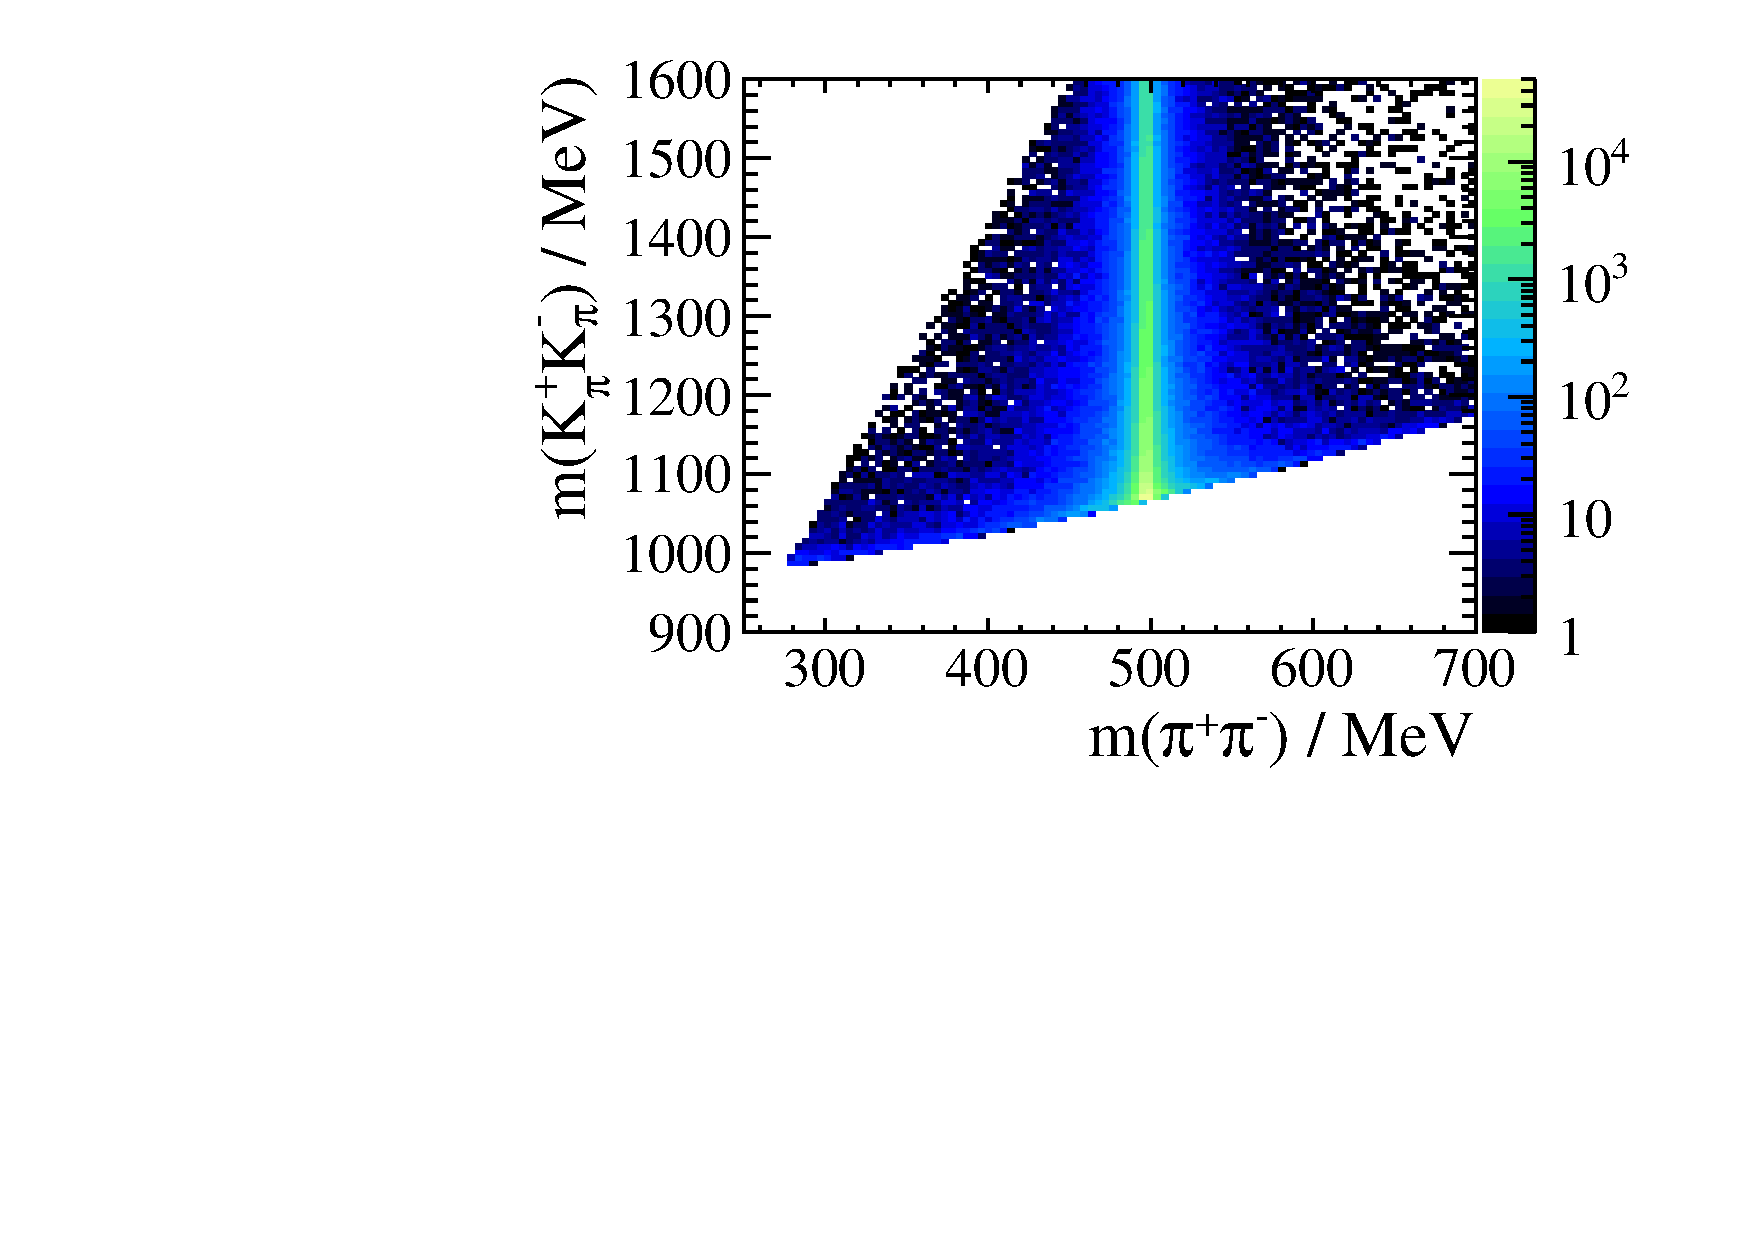
\includegraphics[width=0.48\textwidth]{gen_kk_pipi}
    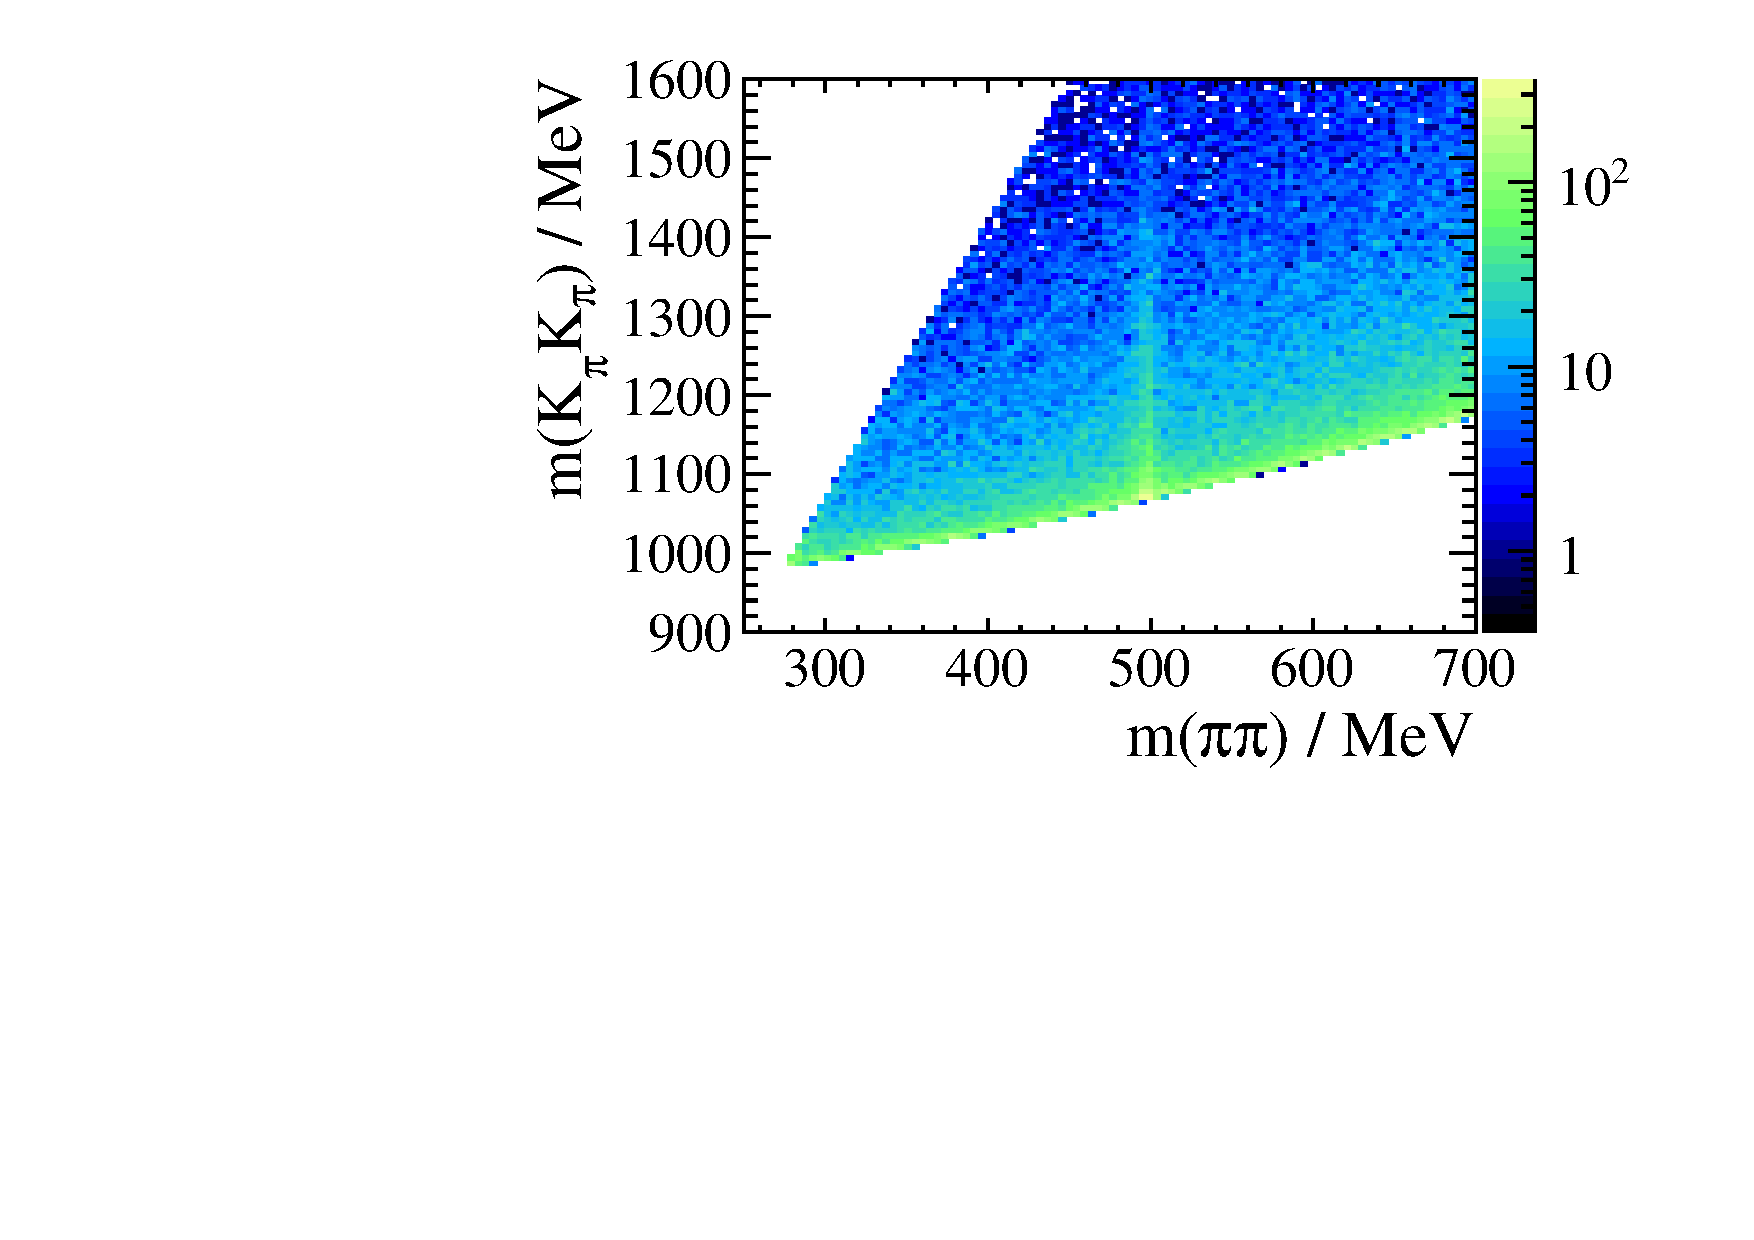
\includegraphics[width=0.48\textwidth]{data_kk_pipi}\\
    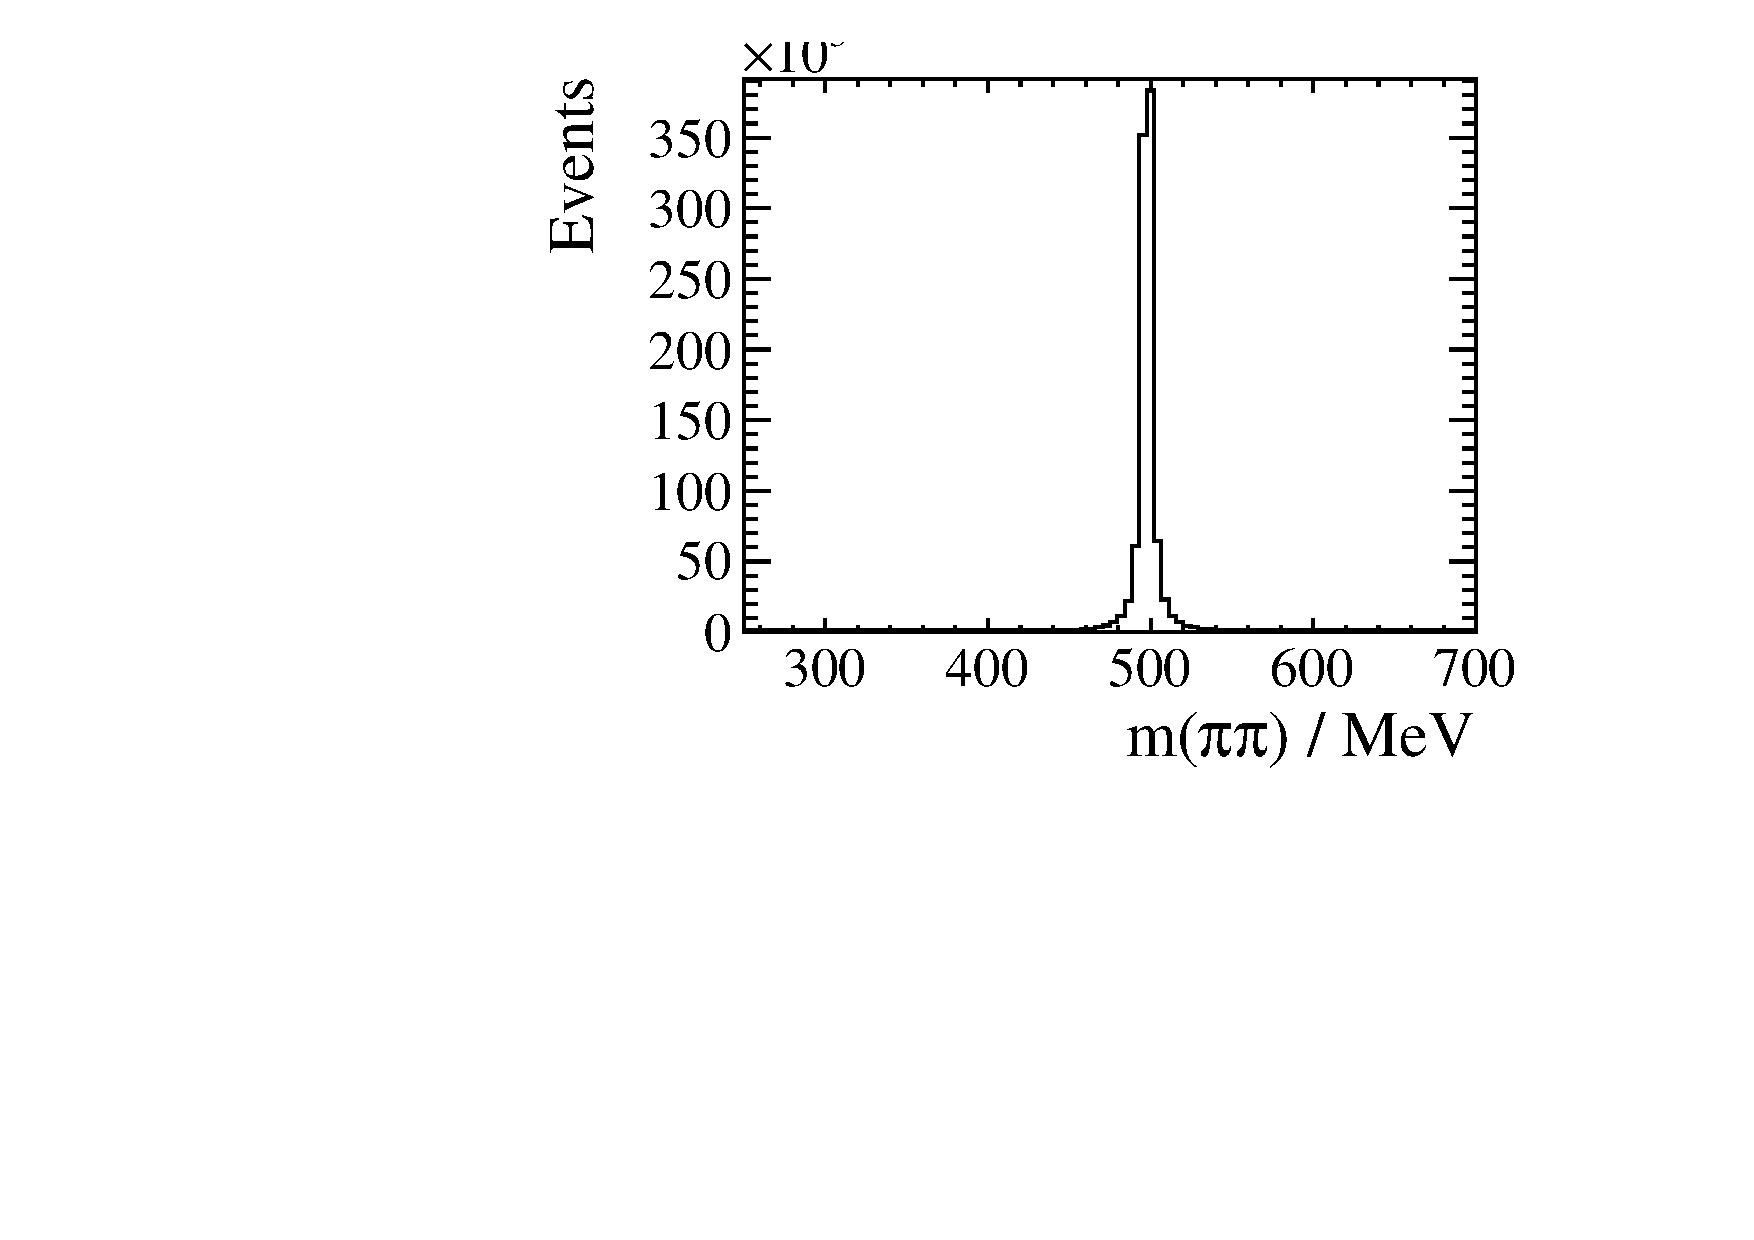
\includegraphics[width=0.48\textwidth]{gen_pipi}
    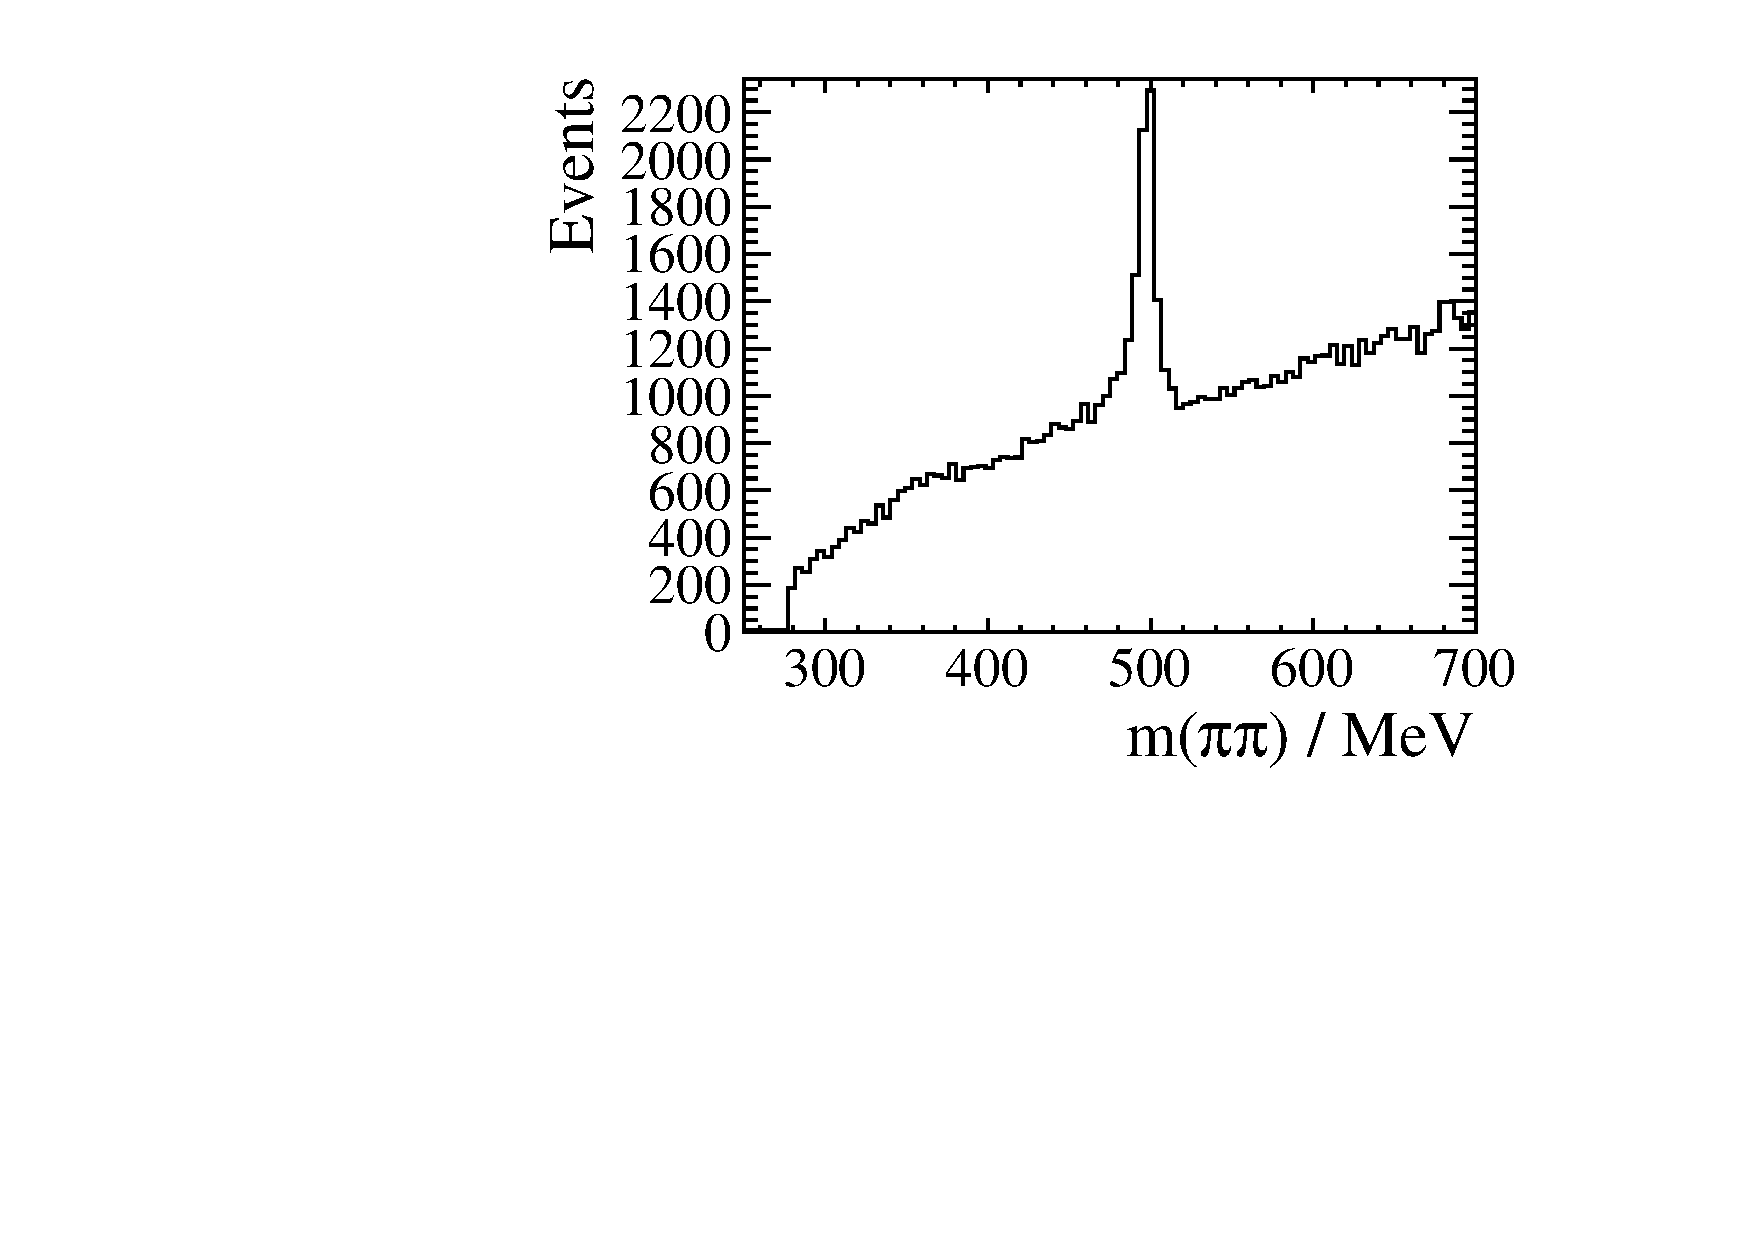
\includegraphics[width=0.48\textwidth]{data_pipi}\\
    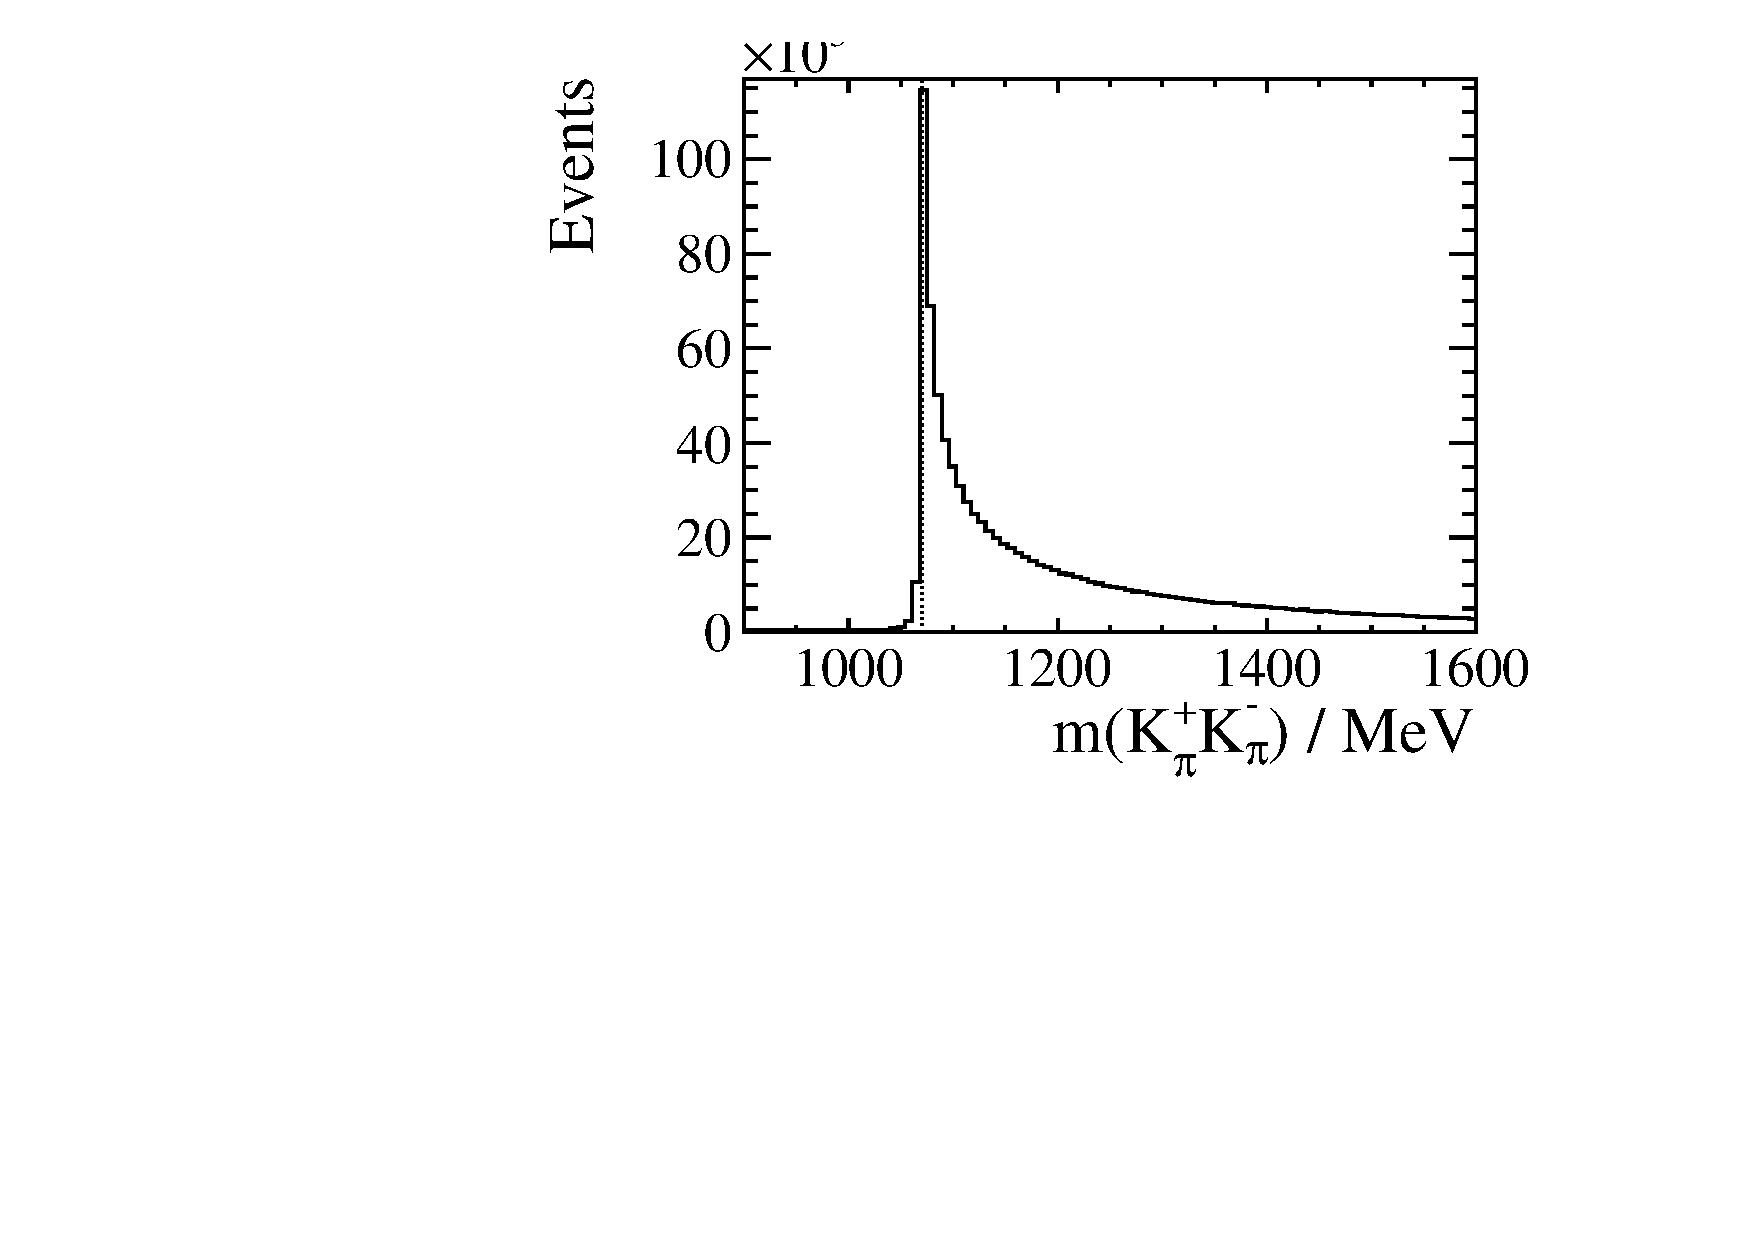
\includegraphics[width=0.48\textwidth]{gen_kk}
    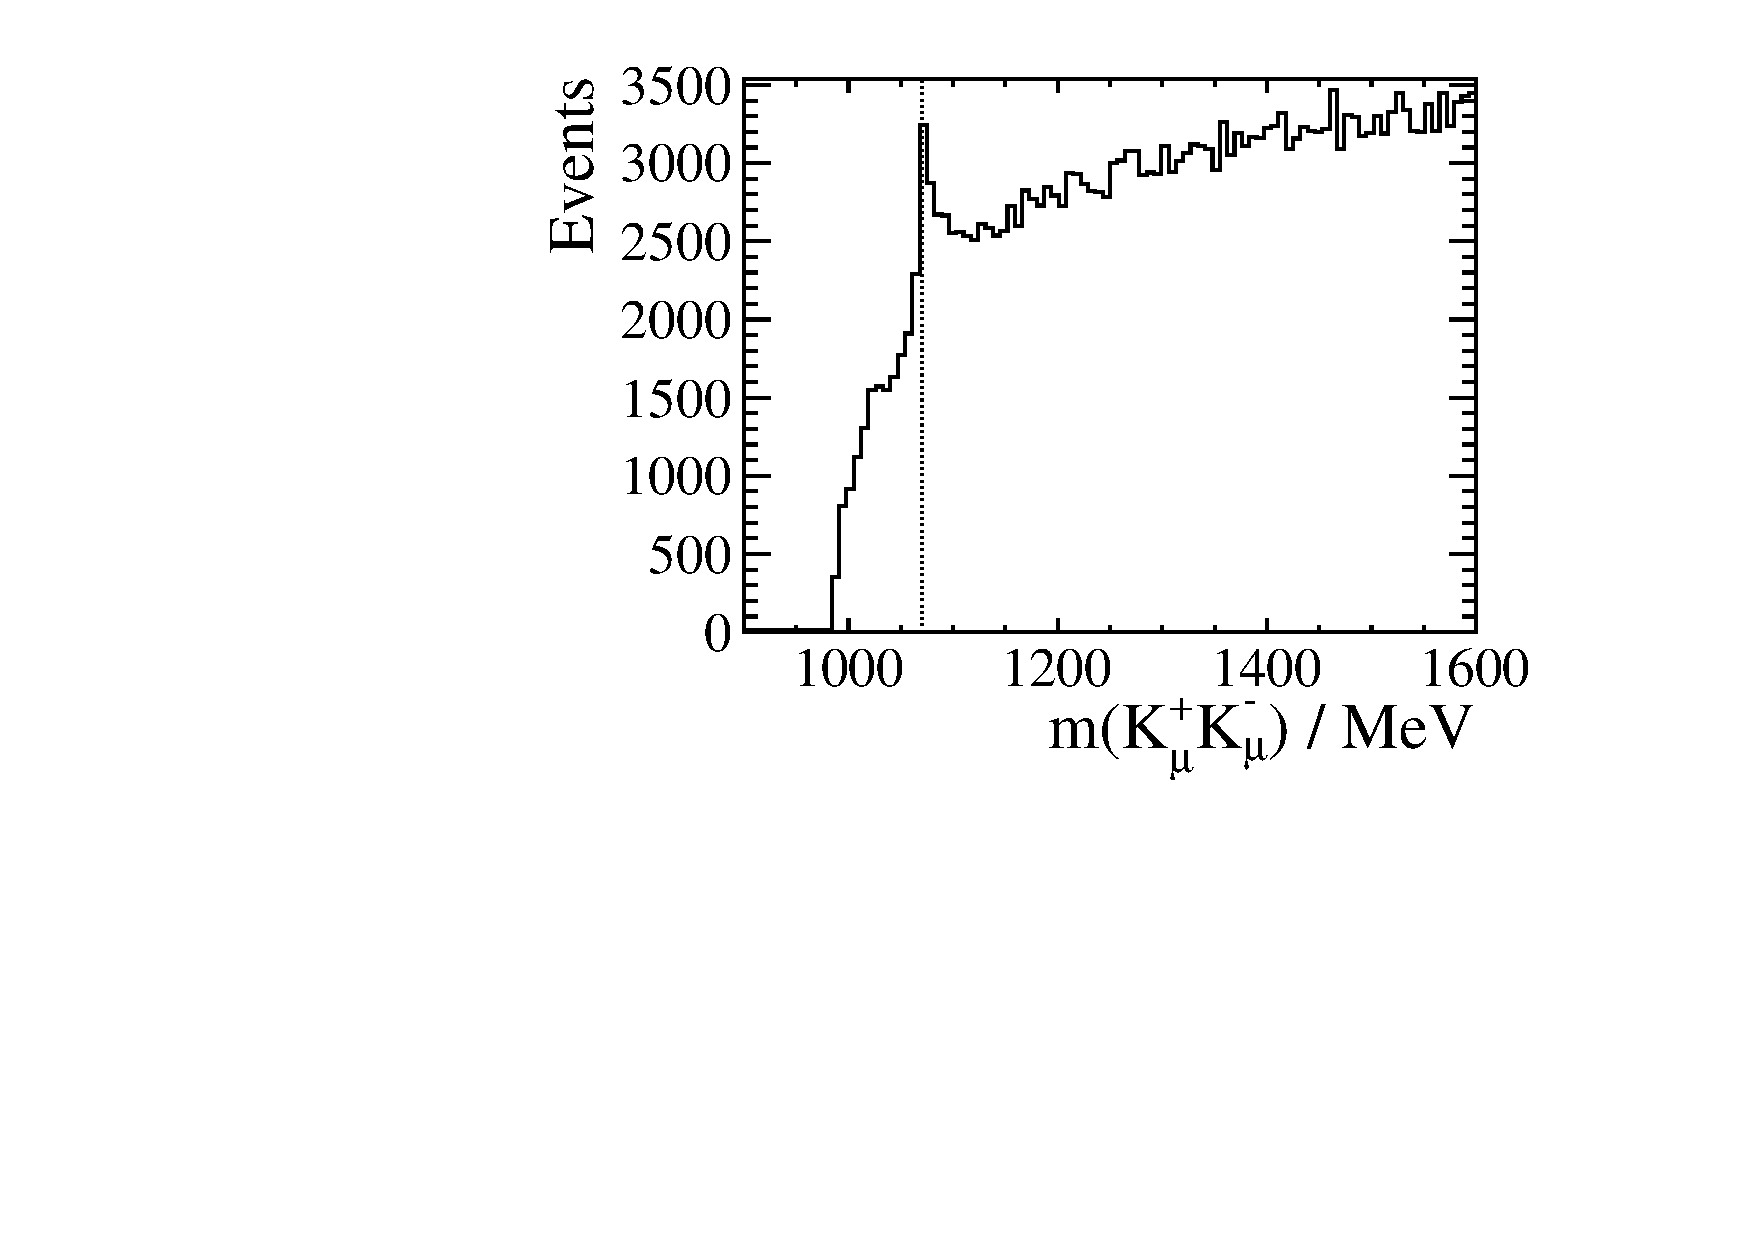
\includegraphics[width=0.48\textwidth]{data_kk}
    \caption[Analysis of the \decay{\KS}{\pipi} background under the \kk mass hypothesis]
    {
      A comparison of \decay{\KS}{\pi\pi} under different mass hypotheses, for
      (left) simulated events, and
      (right) events from data.
      The (top) plots show the two dimensional distributions of the invariant mass distributions of
      a \pipi pair and the same candidates in the \kk mass hypothesis, the (middle) and (bottom)
      plots show the projections.
      Vertical lines in the lower plots indicate $1072\mev$.
    }
    \label{fig:db:x1070:2d}
  \end{center}
\end{figure}


